\section{Evaluation}\label{sec:results}
In diesem Abschnitt werden die Ergebnisse des Experiments vorgestellt.
Dafür wird zunächst das Interview im Zusammenhang mit der Navigation durch die beiden Prototypen beschrieben.
Um einzelne Aussagen von den Teilnehmenden des Experiments zu belegen, werden Aussagen mit der Notation [P$x$, $y$] versehen.
Hierbei steht $x$ für die Nummer der Testperson und $y$ für die Zeile der Aussage im transkribierten Interviewprotokoll.
Im Anschluss werden die Auswertungen der Fragebögen vorgestellt.
Die Ergebnisse wurden mithilfe der Programmiersprache R ausgewertet.
R ist eine Programmiersprache und Umgebung zur statistischen Datenanalyse und anschließender Visualisierung \cite{rlang}.

\subsection{Allgemein}
% Verhalten Recherche
Zunächst werden Ergebnisse, welche sich auf allgemeine Faktoren beziehen, vorgestellt.
Dabei lässt sich festhalten, dass Personen bei ihrem Rechercheverhalten oder der Navigation unterschiedliche Ansprüche und Vorgehensweisen besitzen.
Person 1 beschreibt dabei sehr konkret ihre Vorgehensweise [P1, 28-44].
Zunächst recherchiert diese Person allgemein über ein Thema.
Anschließend werden speziellere Informationen gesucht, welche sich auf das Thema beziehen.
Zuletzt werden Themen, welche indirekt mit dem Thema in Verbindung stehen, recherchiert.
Andere Person tendieren dazu sich Artikel anzusehen, welche einen Bezug zum vorherigen Artikel haben [P3, 116-119; P6, 102-106].
Dabei scheinen diese Personen immer zwei Artikel bezüglich eines Themas zu lesen.
Person 6 begründet dies damit, dass ein Artikel meistens nicht genügt, um ein bestimmtes Thema zu verstehen.\\

%%% Fokus Titel
Durch den Aufbau des Experiments wurde ein verstärkter Fokus der Testpersonen auf die Überschriften der Artikel erzeugt.
Dies spiegelt sich bei sämtlichen Testpersonen darin wider, dass diese die Überschrift in den Vordergrund stellen.
Obwohl dies auf der einen Seite ein realistisches Verhalten abbildet, weil Testpersonen ihrem Interesse folgen, kann dies auf der anderen Seite zu einer Verzerrung der Ergebnisse führen.
Das liegt daran, dass der Fokus auf die Überschriften den Fokus auf die Titel der Artikel verlagert und nicht mehr auf die Navigation.
Vermehrt waren finanzielle oder aktuelle Themen für die Testpersonen interessant.
Person 2 erläutert zusätzlich, dass die Preissteigung von Diesel sie nicht betrifft, da sie keinen Diesel fährt [P2, 54-67].\\

% Clickbait & Werbung
Allgemein wurde das Thema Clickbait von einigen Testpersonen angesprochen [P2, 228-230; P4, 107; P4, 155-158; P5, 5-6; P10, 46-47].
Dieses Thema hat nicht direkt, sondern indirekt, etwas mit der Navigation durch die Prototypen zu tun.
Person 5 macht deutlich, dass sie diese Artikel aus Prinzip nicht klicken würde, wenn es sich um reißerische Überschriften handelt [P5, 5-6].
Person 10 hingegen erwähnt zwar, dass diese Artikel \glqq nichts aussagen\grqq{}, würde diese jedoch trotzdem lesen [P10, 46-47].
Hier wird ebenfalls deutlich, dass die Gruppe von Nutzenden keineswegs homogen ist.
Auch der Aspekt von Werbung in Artikeln wurde von diesen beiden Testpersonen angesprochen [P5, 3-4; P10, 19-21].
Das Problem Clickbait wurde bereits näher in \autoref{subsec:challenges} beschrieben.
Da die Artikel in beiden Prototypen von einer Quelle stammt, welche Klicks von Nutzenden maximieren möchten, spiegelt sich auch der Aspekt von Clickbait in den Artikeln wider.
Werbungen werden aus finanziellen Gründen in Artikeln platziert.
Sie sind einer der Gründe, weswegen die Klicks von Nutzenden als Metrik verwendet werden.

\subsection{Liste}
Während der Navigation durch die Liste ist bei den Testpersonen aufgefallen, dass sie Liste nicht intuitiv als Sortierung nach Ähnlichkeit interpretiert haben.
Auch in diesem Fall sind die Teilnehmenden nach Überschriften von Artikeln vorgegangen, um bei den Aufgaben ähnliche oder unähnliche Artikel zu finden [P2, 250-254].
Dies könnte auf unterschiedliche Arten interpretiert werden.
Zum einen könnte es daran liegen, dass das Experiment keinen ausreichenden Bezug auf andere Listensysteme mit \acp{RS} hat.
Zum anderen könnte es daran liegen, dass die Testpersonen kein allgemeines Verständnis von Listen, welche durch content-based \acp{RS} erstellt werden, haben.
Ebenfalls wurden in zwei Fällen unbekannte Überschriften als unähnlich zu einem vorgegebenen Artikel interpretiert [P3, 68-72; P4, 133-141].\\

% Position Bias
Die in \autoref{subsec:challenges} erwähnte Problematik, dass Listen eine Art von Position Bias mit sich bringen, konnte durch eine Aussage bestätigt werden [P1, 48-53].
Person 1 erwähnte explizit, dass sie die Liste von oben nach unten liest und auch in dieser Reihenfolge konsumiert.
Eine weitere interessante Beobachtung brachte die Reihenfolge in der Personen mit den Prototypen interagieren hervor.
Die erste Aussage von Person 2 war, nachdem sie durch den Begriffsverband navigiert hatte, dass die Liste \glqq relativ zusammenhangslos\grqq{} sei und dass sie keine Form der Kategorisierung erkennt [P2, 202-203].
Sie machte zusätzlich beim Beantworten vom Fragebogen \ac{QUESI}, dass ihr diese Form der Kategorisierung in der Liste gefehlt hat [P2, 262-265].
Im gleichen Satz wurde jedoch auch erwähnt, dass Listen sehr einfach zu verwenden sind.
Dieser Gedanke wird von mehreren Testpersonen geteilt und auch von Person 3 zusammengefasst [P3, 74-78].
Listen sind für die Testpersonen einfach zugänglich und weisen eine geringere Komplexität als ein Begriffsverband auf.\\

% Umdenken 
Die einzigen beiden Personen, welche erwähnten, dass sie nur die Liste privat verwenden würden, waren Person 1 und Person 3.
Person 1 begründet dies damit, dass die Navigation durch den Begriffsverband zu umständlich ist [P1, 388-401].
Die Kategorisierung wird zwar als positiv empfunden, aber die Darstellungsform ist zu unübersichtlich.
Sie erwähnt explizit, dass der Gedanke nicht fallen muss: \glqq In welche Kategorie will ich mich denn jetzt begeben?\grqq{}.
In diesem Fall lässt sich jedoch auch sagen, dass das Experiment auf den ersten Blick erfolgreich war, da bei den Testpersonen ein Umdenken stattgefunden hat.
Schließlich war das Ziel des Experiments, dass Personen sich zuerst Gedanken über die Kategorie machen und sich im Anschluss Artikel aus dieser Kategorie aussuchen.
Dieses müsste jedoch noch weiter verfolgt werden, um eine konkretere Aussage treffen zu können.
Schließlich ist damit noch nicht bewiesen, dass dies auch eine Auseinandersetzung mit kritischeren Inhalten fördert.\\

% Liste simpel
Auch Person 3 erwähnt, dass Listen einfacher zu bedienen sind [P3, 178-184].
Sie möchte vermeiden über die Navigation nachzudenken und stattdessen Optionen präsentiert zu bekommen, welche auf ihre Interessen zugeschnitten sind.
Auch Person 3 erwähnt, dass explizit, dass sie kein Interesse daran hat, sich Gedanken über die Kategorisierung zu machen [P3, 212-214].
Der Grund hierfür liegt darin, dass die Navigation durch die verschiedenen Kategorien zu viel Zeit in Anspruch nehmen würde.
Person 3 bevorzugt es, Inhalte in kurzen Zeitintervallen zu konsumieren, was dazu führt, dass sie weniger Zeit für das Navigieren aufwenden möchte.
In diesem Fall ist eine Listendarstellung dem Begriffsverband vorzuziehen, da die Navigation durch auf Personen zugeschnittene Artikel einen geringeren Zeitaufwand mit sich bringt als das eigenständige Suchen von Artikeln.

\subsection{Begriffsverband}
Das Tutorial wies einige Probleme auf.
Dies konnte, unter anderem, durch die Aufgaben im Tutorial gezeigt werden.
Alle Testpersonen konnten die Anzahl der Gegenstände in der Kategorie pflanzliche Nahrungsmittel korrekt bestimmen.
Jedoch wurde die Gesamtanzahl der Gegenstände bei der Kategorie Nahrungsmittel bei vier Personen falsch beantwortet.
Das Problem daran ist, dass die Testpersonen die Anzahl der Gegenstände in der Kategorie pflanzliche Nahrungsmitteln mit den Gegenständen der Kategorie tierische Nahrungsmittel aufsummiert haben [P2, 17-20; P4, 16-17].
Auf diese Weise wurde jedoch der Gegenstand Rindfleischburger doppelt gezählt.
Zwei der Personen haben zusätzlich zu den genannten Kategorien den Rindfleischburger mit in die Kategorie Nahrungsmittel aufgenommen [P3, 81-85; P5, 7-10].
Auf diese Art und Weise wurde der Rindfleischburger dreifach gezählt.
Dies deutet darauf hin, dass im Tutorial ein Knoten mit implizit gegebenen Merkmalen nicht ausreichend erklärt wurde.
Ebenfalls müsste deutlich gemacht werden, dass Rechenoperationen wie die Addition der Anzahl von zwei Knoten nicht immer möglich sind.
In einem zukünftigen Tutorial könnte es sinnvoll sein die einzelnen Gegenstände aufzuzählen, anstatt die Gesamtanzahl zu bestimmen.
Dies würde das Verständnis der Darstellung im Begriffsverband besser stärker.
Zusätzlich wird die Kompetenz vom Bestimmen einer konkreten Anzahl Testpersonen im Endprodukt nicht benötigt.\\

% Rindfleischburger 
Im Tutorial ist allgemein aufgefallen, dass der Rindfleischburger für die Testpersonen verwirrend war.
Dieser wurde zwar analog zum vorherigem Beispiel mit dem Gegenstand Schwein in \autoref{fig:begriffsverband-tiere} dargestellt, jedoch wurden im Zusammenhang vermutlich zu viele Konzepte gleichzeitig erklärt.
Dies führte dazu, dass in diesem Fall das im Interview eine aktive Erklärung zu diesem Knoten notwendig war.
Dabei wurde die Zusammensetzung eines Rindfleischburgers und die Kategorisierung in tierische und pflanzliche Nahrungsmittel erläutert.
Das aktive Eingreifen ist notwendig gewesen, da ansonsten die Darstellung von Artikeln im Begriffsverband nicht verstanden worden wäre.\\

% Letzte Seite im Tutorial
Für die Teilnehmenden des Experiments war jedoch eindeutig die letzte Seite des Tutorials schwierig.
Diese beinhaltete die Liste, welche nach Anzahl der Welten sortiert war.
Es kamen bei allen Personen, bis auf Person 5 und Person 10, auf, dass diese Seite eine zu hohe Komplexität aufweist.
Vermutlich hat die Erklärung und das von Person 2 erwähnte Problem dazu beigetragen, dass diese Seite als sehr komplex empfunden wurde.
Person 2 erwähnte, dass der zusätzliche Knoten für Verwirrung gesorgt hat [P2, 29-41].
In diesem Fall wäre eine Verbesserung, dass der Knoten mit dem Merkmal Staat nicht aufgetrennt werden sollte.
Dies ist ein Problem, da die Testpersonen die Kompetenz von aufgetrennten Knoten im Tutorial nicht erworben haben.
Stattdessen sollte Schritt für Schritt erklärt werden, wie die Liste sich zusammensetzt.\\

% Zahlenbeispiel
Person 1 erwähnte einen weiteren Verbesserungsvorschlag für das Tutorial.
Sie erwähnte, dass es hilfreich wäre, wenn im gegebenen Beispiel die Anzahl der Gegenstände als Zahl doppelt vorkommen sollen [P1, 123-138].
Der Grund dafür ist, dass es ansonsten zu Fehlinterpretationen kommen kann, da Personen von einer aufsteigenden Nummerierung ausgehen.
Dieses Problem ist, bis auf die kurzzeitige Verwirrung von Person 1, nicht aufgetreten.
Jedoch ist es sinnvoll jegliche Verwirrung zu vermeiden, da dies die Kompetenzen der Testpersonen beeinträchtigen kann.
Ein verwirrendes Tutorial kann dazu führen, dass der Lernerfolg oder die Motivation negativ beeinflusst wird.
Aus diesem Grund sollten jegliche Risiken minimiert werden. \\

% Tutorial = Gut
Trotz einiger Kritikpunkte und Komplikationen wurde das Tutorial als hilfreich empfunden.
Person 2 äußert sich positiv über das Tutorial und ist der Meinung, dass das Tutorial den strukturellen Zusammenhang im Begriffsverband deutlich macht [P2, 182-189].
Ohne das Tutorial müsste sie über Trial-and-Error durch den Begriffsverband navigieren, ohne zu wissen, wie Zusammenhänge im Begriffsverband funktionieren.
Auch an einer anderen Stelle hat das Tutorial eine positive Wirkung.
Zwei Personen nehmen bei der Navigation durch den Begriffsverband zum Tutorial Bezug [P1, 204-205; P3, 99-102].
Dies zeigt, dass Kompetenzen aus dem Tutorial erfolgreich auf die Navigation im Begriffsverband übertragen werden konnten.\\

% Unklare Begriffe
Im Tutorial und auch im Prototyp gibt es ebenfalls Begriffe, welche unklar sind oder für Verwirrung sorgen.
Der Begriff Knoten zum Beispiel ist für Person 6 unklar [P6, 3].
Dieser Begriff sollte im Tutorial zusätzlich erklärt werden, um Personen die Möglichkeit zu geben, sich mit dem Begriff vertraut zu machen.
Zusätzlich sorgt die Benennung der Welt Grün aus den \ac{EC} für mehrdeutige Interpretationen [P4, 50-52].
Grün könnte ebenfalls als die politische Partei der Grünen interpretiert werden.
Da die Begriffe nicht zwangsläufig mit den Begriffen der \ac{EC} übereinstimmen müssen, könnte stattdessen der Begriff Umwelt verwendet werden.
Dies gilt auch für die nicht notwendige Einführung des Begriffs Welt [P1, 171-173].
Dieser Begriff ist nicht notwendig, da Welt im Begriffsverband gleichzusetzen ist mit dem Begriff Kategorie.\\

% Prototyp interessant
Abseits vom Tutorial wird der zugehörige Prototyp als interessant empfunden [P1, 101; P6, 143-148].
Obwohl Testperson 3 die Darstellung als Liste präferiert, ist sie der Meinung, dass die Kategorisierung von Inhalten sinnvoll ist [P3, 190-195].
Ebenfalls wird betont, dass Zusammenhänge im Begriffsverband deutlich werden.
Die Zusammenhänge sollen laut Person 9 im Vergleich zur Liste übersichtlicher sein [P9, 149-150].
Diese Person ist ebenfalls der Meinung, dass die Kategorisierung hilfreich ist, um Zusammenhänge zu verstehen [P9, 105-107].
Sie benennt die Kategorisierung als hilfreich, um zu verstehen, mit welcher Intention ein Artikel geschrieben wurde.
Dieser Gedanke zeigt, dass die Darstellungsform im Begriffsverband die Filterblase für Nutzende des Systems sichtbar macht.
Person 4 illustriert eine weitere positive Eigenschaft der Kategorisierung [P4, 198-203].
Sie erwähnt, dass die Kategorisierung hilfreicher für ein Verständnis ist als nur ein Titel.
Diese Eigenschaft der Kategorisierung fasst laut Person auch auf positive Art und Weise Inhalte zusammen [P5, 134-142].\\

% Artikelansicht intressant
Auch die Artikelansicht im Begriffsverband wird als positiv empfunden [P8, 20-22].
Speziell fehlt jedoch die Möglichkeit, wie im Tutorial, hervorgehobene Textsegmente zu sehen, welche die Kategorisierung von Artikeln in die unterschiedlichen Welten der \ac{EC} verdeutlichen [P3, 99-102; P5, 112-126].
Eine permanente Hervorhebung der Textsegmente könnte den Lesefluss stören.
Aus diesem Grund wäre es sinnvoll, dass die Textsegmente nur bei Bedarf hervorgehoben werden können.
Dies könnte durch einen Toggle-Button realisiert werden.
Person 10 macht darauf aufmerksam, dass es durch die Hervorhebung von Kategorien auch einfacher möglich sein könnte negative Kommentare zu verfassen [P10, 32-36].
Insbesondere, wenn dieses Problem aus politischer Sicht betrachtet wird, könnte es sehr wahrscheinlich sein, dass negative Kommentare bei der gegenüberliegenden politischen Richtung verfasst werden.
Diese Herausforderung sollte bei der Weiterentwicklung des Prototyps berücksichtigt werden.\\

% Farben
Die farbliche Repräsentation von Rechtfertigungen wird von den Teilnehmenden des Experiments als sinnvoll empfunden [P2, 27-28].
Sie ermöglichen und unterstützen unter anderem das Rechercheverhalten von Person 1 [P1, 270-294]. % auch erwähnt, dass es unklar ist
Diese Person präferiert ist sich zunächst positive Rechtfertigungen und im zweiten Schritt negative Rechtfertigungen anzusehen.
Mithilfe dieses Verhaltens kann die Person sich ein Gesamtbild über ein gegebenes Thema machen.
Auch in diesem Fall trägt die Darstellungsform dazu bei, dass die Rechtfertigungen der Artikel deutlich sichtbar werden [P2, 301-307].
Die anteilmäßige Darstellung wird von Person 5 als intuitiv verstanden [P5, 156-160].
Person 6 erweitert diese Aussage und erklärt, dass diese Darstellungsform praktisch und übersichtlich ist [P6, 157-159].
Diese Aussagen deuten darauf hin, dass die Darstellung von Rechtfertigungen im Begriffsverband in der Masterarbeit weniger Probleme bereitet als in der Vorstudie.
Allerdings ist ein eindeutiger Vergleich zwischen der Darstellungsform der Vorstudie und der Masterarbeit erforderlich, um diese Aussage zu bestätigen. \\

% Viel positiv
Ein weiter Vorteil der farblichen Repräsentation ist es ein auf einem Blick ein Gesamtbild über die Rechtfertigungen aller Welten zu erhalten.
Es wird jedoch angemerkt, dass der gegebene Datensatz zu wenig negative Rechtfertigungen enthält [P4, 68-70; P5, 234-236].
Dies muss jedoch nicht zwangsläufig ein Problem sein, da Rechtfertigungen bei realen und größeren Datensätzen nicht zwangsläufig gleichmäßig verteilt sind.
Ein Problem ist jedoch, dass bei einer Interaktion mit der Kategorie die Artikel kein Indiz für die Rechtfertigung einer Welt erhalten.
Dies ist ein Problem, weil Nutzende des Systems nicht erkennen können, ob ein Artikel positiv, negativ oder aus beiden Rechtfertigungen besteht.
Eine Möglichkeit dieses Problem zu lösen wäre, dass die Artikel in der Kategorieansicht eine Farbe erhalten, welche die Rechtfertigung der Welt darstellt [P6, 52-60].
Dies ist jedoch nur möglich, wenn eine Kategorie angeklickt wird, welche nur eine Welt repräsentiert.
Bei Knoten, welche mehr als einer Welt repräsentieren, müssten mehrere Farben verwendet werden, was wiederum die Übersichtlichkeit beeinträchtigen könnte.\\

% Mehrere Merkmale
Bei Knoten mit mehreren Merkmalen gab es unterschiedliche Meinungen.
Person 2 äußerte, dass sie es für sinnvoller hält, wenn die impliziten Merkmale explizit ausgeschrieben werden [P2, 285-295].
Person 5 hingegen ist der Meinung, dass dies nicht notwendig ist und zu viel Text ablenken würde [P5, 176-178].
Diese Meinung bestätigt die in der Masterarbeit vorgeschlagene Lösung, möglichst wenig Text im Begriffsverband zu verwenden, um die Übersichtlichkeit zu erhalten.
Da der Vorschlag von Person 2 jedoch auch seine Berechtigung hat, wurde im Interview spontan eine Lösung für dieses Problem gefunden [P5, 179-182].
Dabei soll das Hovern über einem Knoten die impliziten Merkmale anzeigen.
Auf diese Art und Weise wird die Übersichtlichkeit erhalten und die Informationen sind trotzdem bei Bedarf verfügbar.
Person 5 äußerte eine weitere Meinung in Bezug auf die Merkmale von Knoten [P5, 147-153].
Sie ist der Meinung, dass beim grau färben von Knoten Merkmale weiterhin angezeigt werden sollten.
Der Grund dafür ist, dass Merkmale nicht mehr sichtbar sind und die Nutzenden in die vorherige Ansicht zurückkehren müssen, um sich das Merkmal zu merken.\\

% Liste und Artikelansicht
Bezüglich der Artikel- und Kategorieansicht wurden ebenfalls unterschiedliche Meinungen geäußert.
Meistens wurden beide Ansichten ausprobiert, aber die Kategorieansicht wurde präferiert.
Der Grund hierfür liegt daran, dass die Kategorieansicht für eine bessere Übersicht und weniger Klicks sorgt [P2, 92-100; P4, 71-76].
Die Übersicht wird als besser empfunden, da mehr Artikel als in der Artikelansicht aufgelistet werden.
Dies führt wiederum zu weniger Klicks, da die Nutzenden nicht unbedingt weitere Knoten anklicken müssen, um mehr Artikel einsehen zu können.
Das Problem bei der Kategorieansicht ist jedoch wiederum, dass ähnliche Herausforderungen wie bei einer Liste mit content-based \ac{RS} auftreten.
Bestätigt wird dieser Verdacht dadurch, dass Person 1 auch bei dieser Liste \glqq einfach den Ersten\grqq{} Artikel anklickt [P1, 261-269].\\

% Verständnis
Ähnlich wie bei der Darstellung von Artikeln als Liste gab es auch bei der Darstellung als Begriffsverband Verständnisprobleme.
Das Verständnis für die Funktionsweise des Begriffsverbandes wurde durch unterschiedlichen Aufgaben abgefragt.
Jedoch konnten nur Person 2 und Person 5 ähnliche und unähnliche Artikel anhand der Darstellung im Begriffsverband finden [P2, 162-177; P5, 197-208].
Alle anderen Personen versuchten die Artikel anhand der Überschriften zu unterscheiden.
Dies ist teils gelungen, jedoch wird dies nicht beachtet, da keine Erklärung anhand der Darstellung erfolgt ist.
Beide Personen, welche die Aufgabe erfolgreich gelöst haben, hatten im Informatikstudium mehrfach Kontakt mit Graphen.
Aus diesem Grund ist nicht auszuschließen, dass einige Kompetenzen, im Vergleich zu anderen Personen, auf den Begriffsverband übertragen wurden. \\

% Übergeordneter Knoten
Dies heißt jedoch nicht im Umkehrschluss, dass die anderen Teilnehmenden keine Kompetenzen im Umgang mit dem Begriffsverband besitzen.
Um Artikel im Begriffsverband zu finden, haben einige Testpersonen den obersten Knoten im Graphen verwendet, um alle Artikel aufzulisten [P1, 329-333; P3, 132-135; P4, 80-82; P10, 58].
Gerade diese Tatsache zeigt ein Verständnis der Testpersonen für den Umfang eines Begriffs.
Person 2 geht sogar einen Schritt weiter und benennt den obersten Knoten als Elektromobilität [P2, 43-45].
Dies ist ein interessanter Aspekt, da die Elektromobilität nur ein Thema von vielen unterschiedlichen Themen ist, welche mit einem Begriffsverband abgebildet werden können.
Das Experiment zeigt nur einen kleinen Ausschnitt aus allen möglichen Themen, welche journalistisch abgedeckt werden.
In einem Interview ist das Konzept des Teilverbandes gefallen [P4, 179-188].
Ein Teilverband ist eine Teilmenge eines Verbandes, welche selbst ein Verband ist.
In diesem Fall könnte Elektromobilität ein Teilverband von Mobilität sein, welches wiederum ein Verband von Verkehr sein könnte.
Dieses Konzept ist nicht Teil der Masterarbeit, aber könnte eine interessante Erweiterung des Begriffsverbandes für weitere Prototypen darstellen.

\subsection{AttrakDiff}\label{subsec:results-attrakdiff}
Für die Visualisierung wurden die Ergebnisse der Online-Plattform vom AttrakDiff verwendet.
Bei der Interpretation der Ergebnisse ist zu beachten, dass alle Personen bereits Vorerfahrung mit der Listendarstellung hatten.
Der Begriffsverband hingegen ist für alle Teilnehmenden ein neues Konzept.

\begin{figure}[!ht]
    \centering
    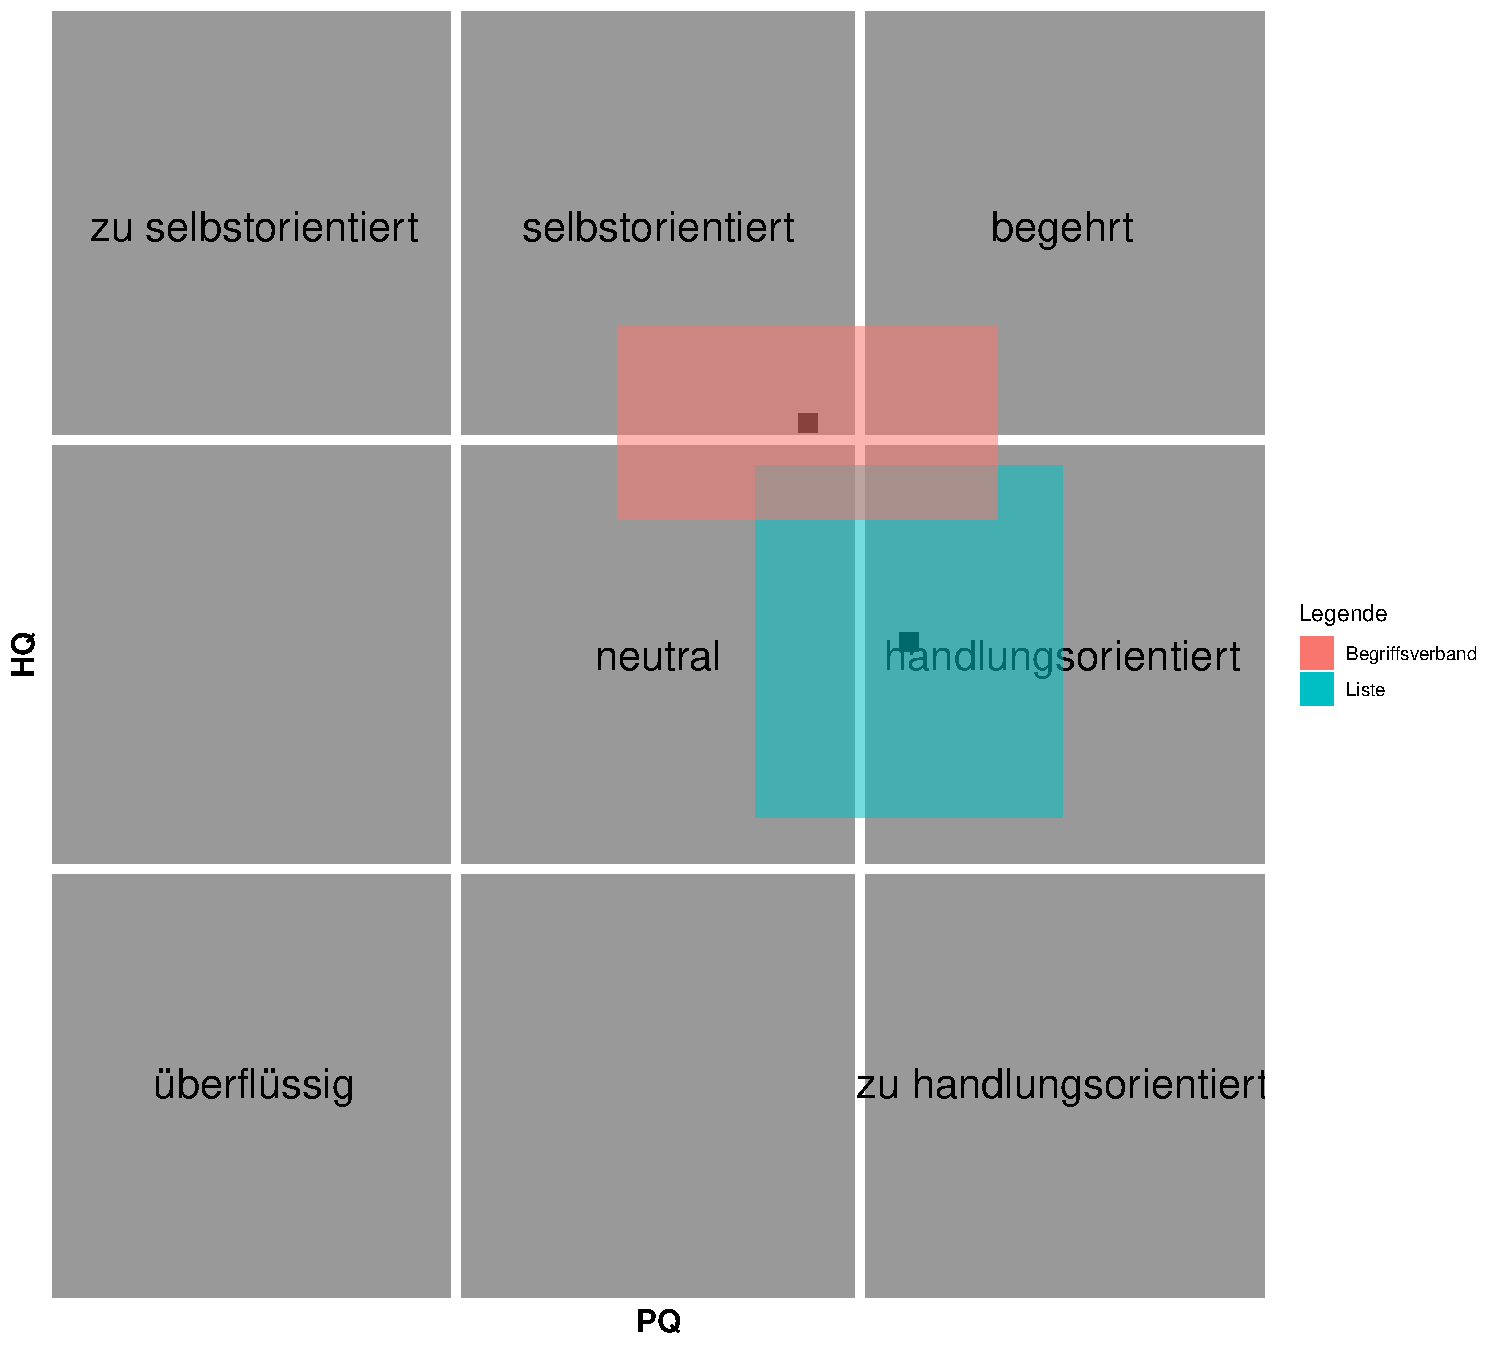
\includegraphics[width=0.7\columnwidth]{figures/attrakdiff-squares.pdf}
    \caption{\label{fig:attrakdiff-squares}AttrakDiff - Portfolio-Darstellung}
\end{figure}

% Portfolio
In \autoref{fig:attrakdiff-squares} werden die Ergebnisse des Fragebogens als Portfolio-Darstellung repräsentiert.
Die einzelnen Quadranten stellen dabei die Relation zwischen \ac{PQ} und der \ac{HQ} dar.
Dabei wird ein Produkt als überflüssig bewertet, wenn es eine niedrige \ac{PQ} und eine niedrige \ac{HQ} hat.
Begehrt ist ein Produkt dann, wenn es eine hohe \ac{PQ} und eine hohe \ac{HQ} hat.
Dazwischen existieren weitere Zustände, welche Kompromissformen zwischen beiden Qualitäten darstellen.
Die Spanne für beide Achsen liegt im Intervall von $-3$ bis $3$. \\

% Konfidenzintervalle
Für beide Werte \ac{PQ} und \ac{HQ} sind Konfidenzintervalle als Rechtecke angegeben.
Diese Rechtecke geben mit einer Wahrscheinlichkeit von $95\%$ an, dass in einer weiteren Umfrage die gleiche oder eine ähnliche Bewertung der Produkte erzielt wird.
Die Rechtecke geben zusätzlich an wie unterschiedlich die Testpersonen die Produkte hinsichtlich der \ac{PQ} und der \ac{HQ} bewertet haben.
Der Unterschied zwischen beiden Produkten ist nicht signifikant, da sich die Rechtecke in der horizontalen und vertikalen Achse überlappen.
Ebenfalls können Produkte nicht eindeutig einem Quadranten zugeordnet werden, da die Rechtecke sich nicht vollständig in einem Quadranten befinden.
Dies liegt daran, dass die Testpersonen die Produkte unterschiedlich wahrgenommen und bewertet haben.
Zusätzlich sorgt die geringe Anzahl der Testpersonen für eine geringere Aussagekraft der Ergebnisse.

\begin{figure}[!ht]
    \centering
    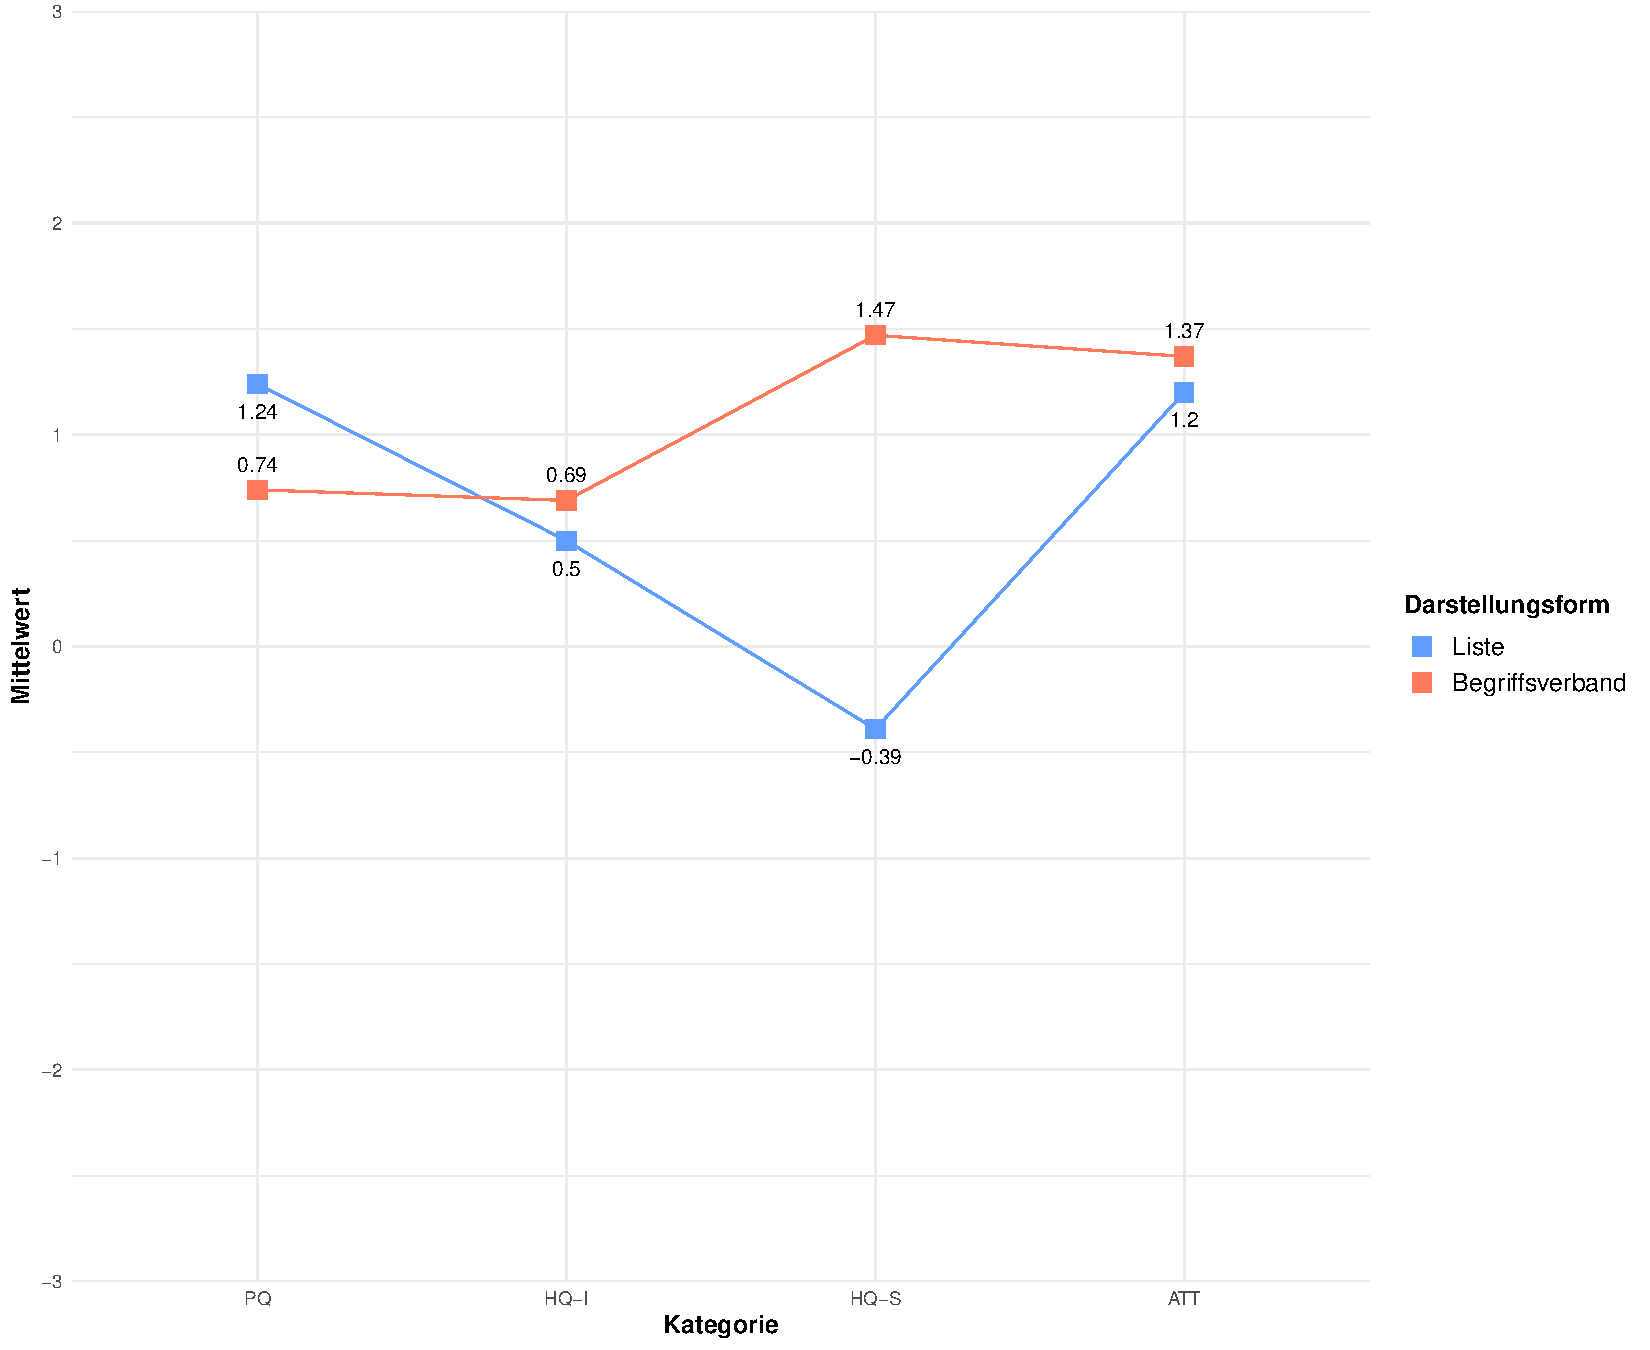
\includegraphics[width=0.7\columnwidth]{figures/attrakdiff-line.pdf}
    \caption{\label{fig:attrakdiff-line}AttrakDiff - Diagramm der Mittelwerte}
\end{figure}

% Mittelwerte
Wenn man die unterschiedlichen Kategorien in \autoref{fig:attrakdiff-line} im direkten Vergleich betrachtet, lässt sich erkennen, dass die Liste nur in der \ac{PQ} im Mittel besser bewertet wurde.
Die \ac{HQ-I}, \ac{HQ-I} und die Attraktivität wurden beim Begriffsverband im Mittel besser bewertet.
Dabei könnte ein Grund für eine bessere \ac{PQ} bei der Listendarstellung sein, dass bereits Vorerfahrungen mit der Handhabung des Produkts bestehen.
Schließlich sind Handlungsziele zu erreichen stark mit dem Vorwissen der Testpersonen verbunden.
Nichtsdestotrotz liegt es ebenfalls nahe, dass die Liste einfacher aufgrund der geringeren Komplexität einfacher zu bedienen ist.\\

% HQ-I und HQ-S
Gerade die \ac{HQ-I} und die \ac{HQ-S} sind für die Untersuchung der Masterarbeit von großer Bedeutung.
Schließlich zeigt besonders die \ac{HQ-S}, dass der Begriffsverband das persönliche Wachstum der Testpersonen besser unterstützt als die Listendarstellung.
\textcolor{red}{TODO: Weiter beschreiben}

\subsection{QUESI}
Mithilfe von R wurden die fünf unterschiedlichen Subskalen vom \ac{QUESI}-Fragebogen ausgewertet.
Dafür wurde das arithmetische Mittel $\overline{x}$ und die Standardabweichung SD berechnet.
Da die Antworten auf einer 5-Punkte Likert Skala gegeben wurden, liegt der Mittelwert zwischen $1$ und $5$.
Die daraus resultierenden Werte sind in \autoref{table:quesi-list} und \autoref{table:quesi-fca} dargestellt.
Zusätzlich wurde der \ac{QUESI}-Score über alle Fragen hinweg als Mittelwert berechnet.
Dieser ist ebenfalls in der Tabelle als Score angegeben und dient als Gesamtbewertung der Testpersonen.

\begin{center}
    \begin{table}[!ht]
        \centering
        \begin{tabular}{|l|c|c|c|c|c|c|}
            \hline
                                                 & Arbeitsbelastung & Ziele & Lernen & Vertrautheit & Fehler & Score \\ \hline \hline
            \multicolumn{1}{|c|}{$\overline{x}$} & 4,4              & 4,4   & 4,7    & 4,67         & 5      & 4,61  \\ \hline
            \multicolumn{1}{|c|}{SD}             & 0,93             & 0,81  & 0,79   & 0,66         & 0      & 0,77  \\ \hline
        \end{tabular}
        \caption{QUESI - Liste}
        \label{table:quesi-list}
    \end{table}
\end{center}

% Mittelwerte QUESI
Die Mittelwerte für \autoref{table:quesi-list} liegen im Bereich von $4,4$ bis $5$.
Dies deutet darauf hin, dass die Testpersonen die Darstellung als Liste als intuitiv empfunden haben.
Während der Verwendung des Systems gab es keine Probleme mit der Bedienung.
Dies zeigt sich dadurch, dass die Standardabweichung bei der Subskala für Fehler bei $0$ liegt.
Allgemein lässt sich sagen, dass die Antworten der Testpersonen sehr einheitlich waren, da die Standardabweichung bei allen Skalen unter $1$ liegt.

\begin{center}
    \begin{table}[!ht]
        \centering
        \begin{tabular}{|l|c|c|c|c|c|c|}
            \hline
                                                 & Arbeitsbelastung & Ziele & Lernen & Vertrautheit & Fehler & Score \\ \hline \hline
            \multicolumn{1}{|c|}{$\overline{x}$} & 3,23             & 4,37  & 3,27   & 3,83         & 4,25   & 3,76  \\ \hline
            \multicolumn{1}{|c|}{SD}             & 1,41             & 0,76  & 1,39   & 1,29         & 0,85   & 1,27  \\ \hline
        \end{tabular}
        \caption{QUESI - Begriffsverband}
        \label{table:quesi-fca}
    \end{table}
\end{center}

% Begriffsverband wenig intuitiv
Bei der Auswertung der Antworten bezüglich des Begriffsverbandes lässt sich in \autoref{table:quesi-fca} erkennen, dass die Testpersonen die Darstellung als Begriffsverband als weniger intuitiv empfunden haben.
Ebenfalls waren die Meinungen der Testpersonen unterschiedlicher als bei der Liste.
Dies zeigt sich darin, dass die Standardabweichung bei mehreren Subskalen über $1$ liegt.
Ein Grund hierfür könnte sein, dass die Testpersonen viel unterschiedlichere Erfahrungen mit dem Begriffsverband gemacht haben.
Beweisen lässt sich dies durch die unterschiedlichen Aussagen und Verständnisse zum Begriffsverband in den Interviews.\\

% Vorerfahrung
Im direkten Vergleich lässt sich sagen, dass die Ziele mit dem Begriffsverband ähnlich gut erreicht werden können wie mit einer Liste.
Wenn man dies mit der \ac{PQ} aus \autoref{subsec:results-attrakdiff} vergleicht, bestätigen sich die Ergebnisse.
Es wird bei der Listendarstellung zwar eine höhere \ac{PQ} erzielt, jedoch ist diese nicht signifikant.
Ebenfalls bestätigen die Ergebnisse vom \ac{QUESI}-Fragebogen, die Annahme, dass die Vorerfahrung mit einem Produkt die \ac{PQ} beeinflusst.
Gerade die Subskalen für Arbeitsbelastung und Vertrautheit fallen beim Begriffsverband deutlich schlechter aus als bei der Liste.
Dies ist jedoch offensichtlich, wenn die meisten Darstellungsformen im Internet als Liste dargestellt werden.\\

% Fehler
Einige Personen gaben an, dass sie Fehler oder Probleme im Begriffsverband wahrgenommen haben.
Das kann daran liegen, dass die Testpersonen nicht die Möglichkeit hatten, sich ausreichend mit dem Begriffsverband vertraut zu machen.
Aus diesem Grund könnte eine hohe Komplexität und Unverständnis bei der Navigation im Begriffsverband die Ursache für schlechtere Ergebnisse sein.
Dieser Wert lässt sich ebenfalls durch die Interviews und die darin enthaltenen Aussagen bestätigen.
Es wäre jedoch möglich, dass der \ac{QUESI}-Score mit zusätzlichen Erfahrungen und einem verbesserten Tutorial beim Begriffsverband steigen würde.

\subsection{Eigener Fragebogen}
In diesem Abschnitt erfolgt die Auswertung der Ergebnisse des selbst erstellten Fragebogens sowie die Analyse der Aufgaben zur Navigation durch die Prototypen.
Jeder Testperson ist nur die Liste oder eine Variation davon als Darstellungsform für Online-News-Artikel bekannt.
Variationen sind hierbei unendliche Listen oder ein zweidimensionales Kachel-Layout.
Beim zweidimensionalen Kachel-Layout wäre es auch möglich von einem eigenen System zu sprechen, da bei dieser Darstellungsform ebenfalls eine Form der Kategorisierung stattfindet.
Die Kategorisierung erfolgt in diesem Fall jedoch nicht nach den \ac{EC}, sondern nach typischen Rubriken wie Sport oder Wirtschaft.\\

\begin{figure}[!ht]
    \centering
    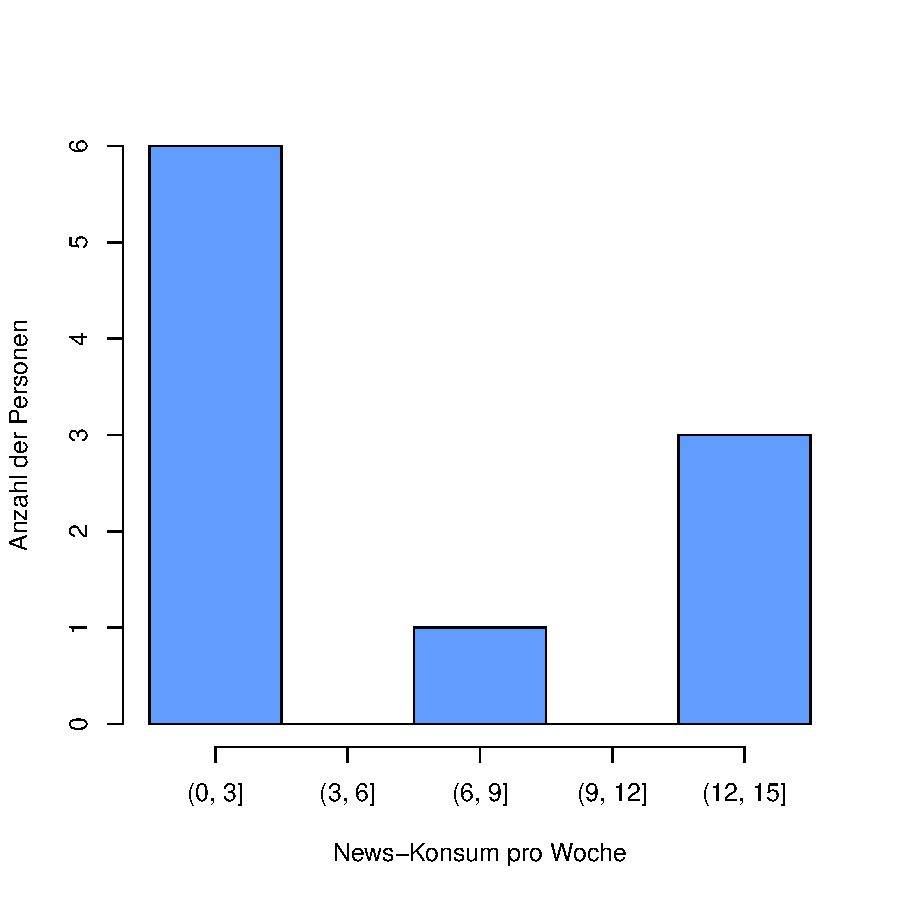
\includegraphics[width=0.6\columnwidth]{figures/news-frequency.pdf}
    \caption{\label{fig:news-consumption}Histogramm - Online-News-Konsum pro Woche}
\end{figure}

% Online-News-Konsum
\autoref{fig:news-consumption} zeigt die Verteilung der Antworten der Testpersonen bezüglich ihres Online-News-Konsums.
Das Histogramm gibt Aufschluss darüber wie stark das Bedürfnis der Testpersonen nach Online-News ist.
Personen mit einem hohen Konsum können als besonders informiert oder interessiert an Online-News angesehen werden.
Ebenfalls kann diese Zielgruppe als erfahren mit der Nutzung von Online-News betrachtet werden.
Dies fällt besonders auf, wenn man den \ac{QUESI}-Score von Personen mit einem täglichen Konsum mit dem Score von Personen mit geringerem Konsum vergleicht.
Bei der Darstellung als Liste ist der Unterschied zwischen den beiden Gruppen groß genug, um als signifikant angesehen zu werden.
Jedoch ist der Unterschied bei der Darstellung als Begriffsverband deutlich größer.
Die Gruppe mit einem täglichen Konsum weist eine geringere mentale Arbeitsbelastung ($\overline{x} = 3,75$) und eine höhere Vertrautheit ($\overline{x} = 4,17$) auf als die Gruppe mit einem geringeren Konsum ($\overline{x} = 2,89$ und $\overline{x} = 3,61$).
Dadurch ergibt sich für die erste Gruppe auch ein höherer \ac{QUESI}-Score ($\overline{x} = 4,12$, SD=$0,90$) als für die zweite Gruppe ($\overline{x} = 3,51$, SD=$1,42$). \\

% Daten schwierig auszuwerten
Vorerfahrung zum Thema E-Mobilität ist nur bei Person 1 vorhanden.
Alle anderen Personen haben, bis auf einige Berichte, keine nennenswerte Vorerfahrung mit dem Thema.
Genau die Hälfte der Testpersonen hat bereits Vorerfahrungen mit Graphen.
Jedoch lässt sich weder aus dieser Vorerfahrung noch aus der Tatsache, dass einige Informatiker unter den Testpersonen waren, sinnvolle Aussagen über die Navigation im Begriffsverband ableiten.
Es ist positiv zu vermerken, dass die Testpersonen den Begriffsverband als eine diverse Darstellung zum Thema E-Mobilität empfunden haben.
Verbunden mit den Ergebnissen aus den Interviews bietet der Begriffsverband eine gute Möglichkeit Zusammenhänge und Beziehungen besser zu verstehen.
Für das Experiment bedeutet dies, dass der Begriffsverband Testpersonen eine bessere Möglichkeit bietet, sich mit dem Thema E-Mobilität kritisch auseinanderzusetzen. \\

% Navigation Aufgabe
Dies lässt sich auch an den Ergebnissen der Aufgaben zur Navigation durch die Prototypen erkennen.
Um die Daten auszuwerten werden die Kreuztabellen aus \autoref{table:list-worlds} und \autoref{table:fca-worlds} verwendet.
Zu Interpretationszwecken wird die Inzidenzrelation dabei als boolesche Variable gelesen.
Das heißt, dass ein Kreuz $\times$ als eine Eins und eine leere Zelle als eine Null interpretiert wird.
Auf diese Weise lässt sich die Inzidenzrelation als binäre Matrix darstellen.
Beim Experiment wurden pro Person je fünf Artikel je Prototyp festgehalten.
Das bedeutet, dass für jede Testperson die Inzidenzrelation eine 5x8 Matrix ist.
Die Zeilen entsprechen dabei den Artikeln und die Spalten entsprechen den unterschiedlichen Welten der \ac{EC}.
Für Testperson 1 sieht die Matrix für den Listen-Prototyp wie folgt aus:

\setcounter{equation}{0}
\begin{equation}
    \begin{matrix}
        1 & 0 & 1 & 0 & 1 & 0 & 1 & 0 \\
        1 & 0 & 1 & 0 & 1 & 0 & 1 & 0 \\
        1 & 0 & 0 & 0 & 0 & 0 & 0 & 0 \\
        0 & 0 & 0 & 1 & 0 & 0 & 0 & 0 \\
        1 & 0 & 1 & 0 & 0 & 1 & 1 & 0 \\
    \end{matrix}
\end{equation}

% Hamming-Distanz
Diese Matrix kann nun verwendet werden, um die Hamming-Distanz zwischen den Welten zu berechnen.
Die Hamming-Distanz ist eine Metrik, welche die Anzahl unterschiedlicher Elemente zwischen zwei Codewörtern misst \cite{hamming-code}.
In diesem Fall wird die Hamming-Distanz zwischen den Welten berechnet.
Dabei gibt diese an wie viele der Welten sich pro Artikel unterscheiden.
Im Begriffsverband sieht die Navigation für Person 1 wie folgt aus:
\begin{equation}
    \begin{array}{ccccccccc}
        1                  & 0 & 1 & 0                  & 0                  & 0                  & 0                  & 0 &                                              \\
        1                  & 0 & 1 & 0                  & 0                  & 0                  & 0                  & 0 & \multicolumn{1}{r}{\quad\textcolor{blue}{0}} \\
        1                  & 0 & 1 & 0                  & 0                  & \textcolor{red}{1} & \textcolor{red}{1} & 0 & \multicolumn{1}{r}{\quad\textcolor{blue}{2}} \\
        1                  & 0 & 1 & 0                  & \textcolor{red}{1} & \textcolor{red}{0} & 1                  & 0 & \multicolumn{1}{r}{\quad\textcolor{blue}{2}} \\
        \textcolor{red}{0} & 0 & 1 & \textcolor{red}{1} & \textcolor{red}{0} & 0                  & \textcolor{red}{0} & 0 & \multicolumn{1}{r}{\quad\textcolor{blue}{4}} \\
    \end{array}
    \label{eq:hamming-distance}
\end{equation}

% Farben Matrix
In \autoref{eq:hamming-distance} sind die Unterschiede zwischen den Welten und die daraus resultierende Hamming-Distanz farblich hervorgehoben.
Die Farbe Rot zeigt an, dass sich ein Artikel zum vorherigen an der markierten Stelle unterscheidet.
In Blau ist die Anzahl der roten Zellen pro Zeile angegeben.
Die erste Zeile hat immer eine Hamming-Distanz von null, da es keinen vorherigen Artikel gibt.
Die Hamming-Distanz der zweiten Zeile ist in diesem Fall ebenfalls null, da sich der Artikel hinsichtlich der Welten nicht vom ersten unterscheidet.
In der dritten Zeile gibt es den ersten Unterschied zum vorherigen Artikel.
Dieser Unterschied ist in Spalte 5 und 6 aufzufinden.
Dieser Artikel weist im Vergleich zum vorherigen Artikel die Merkmale Staat- und Grün\texttt{+} auf.\\

\begin{figure}[ht!]
    \centering
    \subfloat[\centering Liste]{{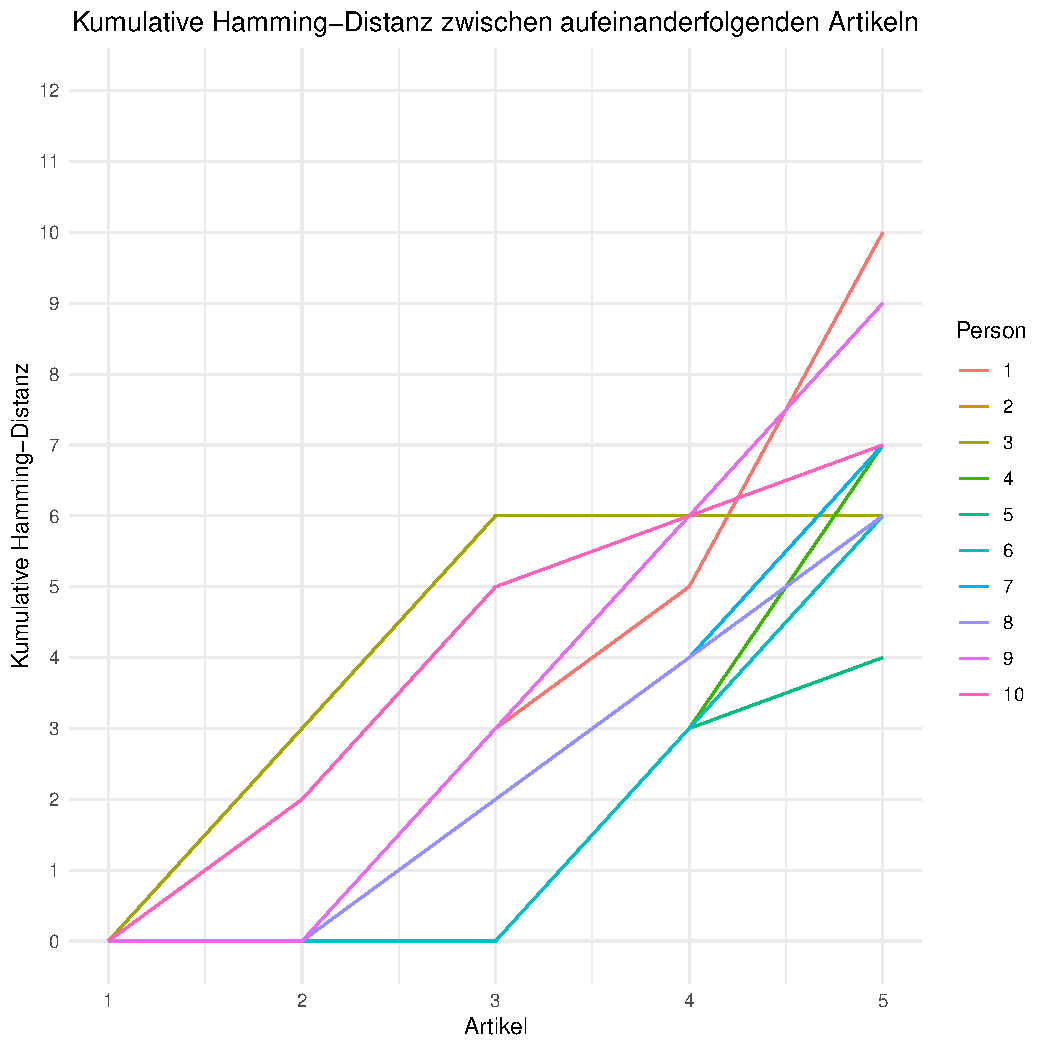
\includegraphics[width=6cm]{figures/list-line.pdf} }}%
    \qquad
    \subfloat[\centering Begriffsverband]{{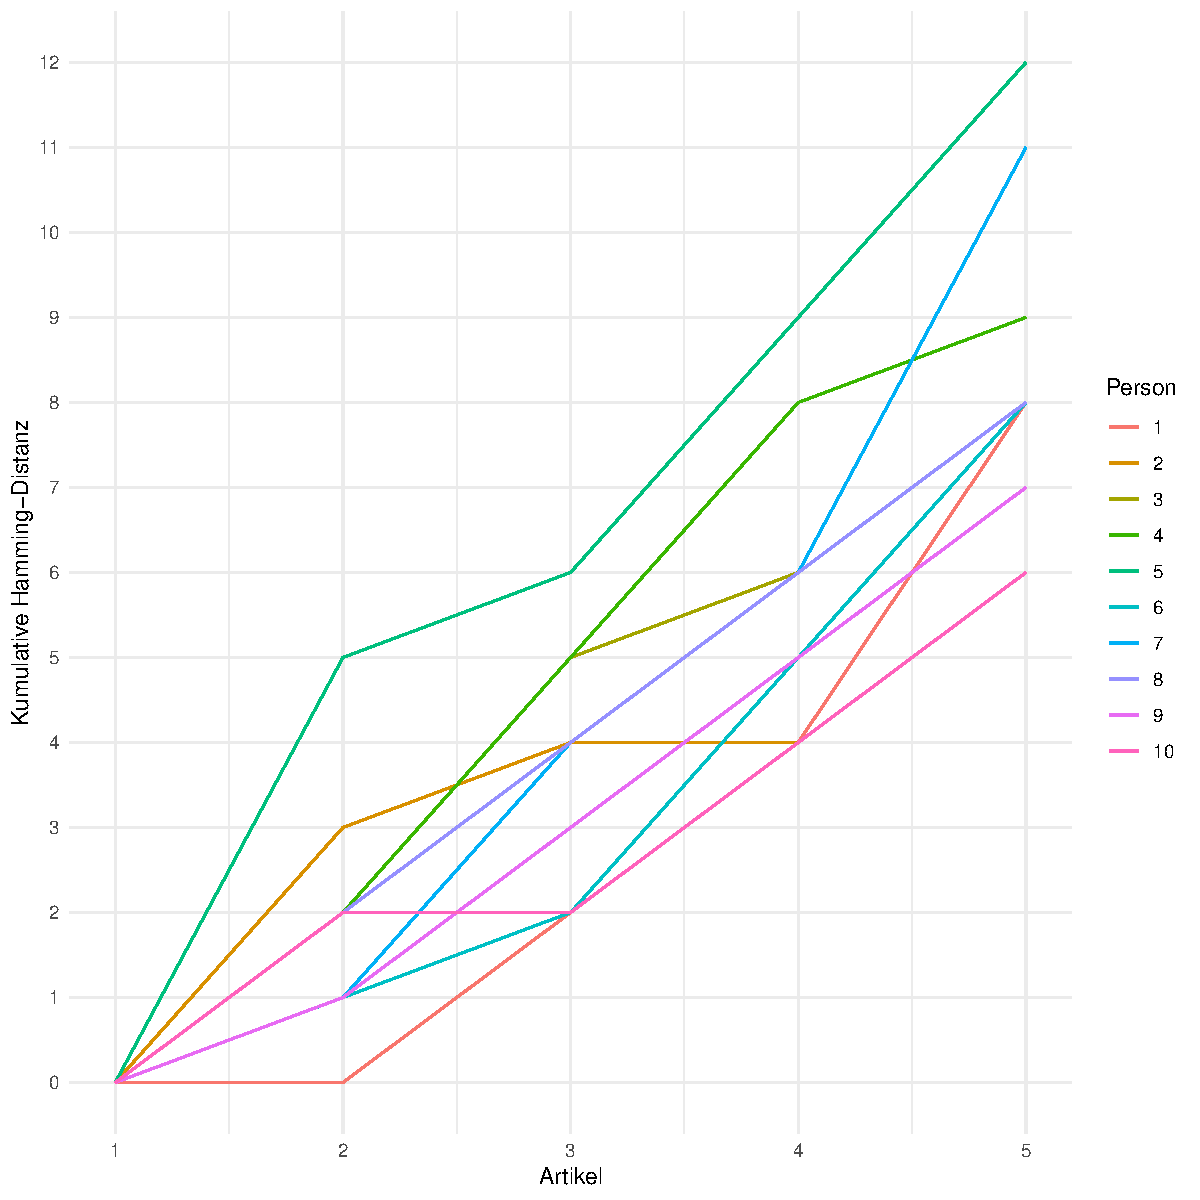
\includegraphics[width=6cm]{figures/fca-line.pdf} }}%
    \caption{Liniendiagramme - Vergleich Hamming-Distanz}
    \label{fig:hamming-distance}
\end{figure}

% Kumulative Hamming-Distanz
\autoref{fig:hamming-distance} stellt im Vergleich die kumulative Hamming-Distanz für die beiden Prototypen dar.
Die kumulative Hamming-Distanz ergibt sich aus der Summe der Hamming-Distanzen aller zuvor geklickten Artikel einer Testperson.
In \autoref{eq:hamming-distance} ist die kumulative Hamming-Distanz für Person 1 gleich acht, da $0 + 2 + 2 + 4 = 8$.
Diese schrittweise Summierung lässt sich auch am Liniendiagramm in \autoref{fig:hamming-distance} ablesen.
Dabei stellt die x-Achse den aktuell gelesenen Artikel dar, welcher in der Matrix als Zeile repräsentiert wird.
Die y-Achse stellt die bis zum gelesenen Artikel aufsummierte Hamming-Distanz dar.\\

% Diversitätsmaß
Die kumulative Hamming-Distanz kann als Diversitätsmaß für die gelesenen Artikel interpretiert werden.
Eine höhere kumulative Hamming-Distanz lässt sich gleichsetzen mit einer höheren Diversität aller gelesenen Artikel.
Auffällig ist hierbei in \autoref{fig:hamming-distance}, dass die kumulative Hamming-Distanz für den Begriffsverband einen höheren Minimal- und Maximalwert aufweist.
Basierend auf dieser Interpretation als Diversitätsmaß kann festgestellt werden, dass der Begriffsverband im Vergleich zum anderen Prototypen zu einer höheren Diversität bei der Navigation durch die Artikel geführt hat.
Es ist ebenfalls zu erkennen, dass bei der Liste das Diversitätsmaß erst beim Lesen des dritten Artikels ansteigt.
Dies würde dafür sprechen, dass Personen durch die Positionierung in der Liste dazu verleitet wurden die Artikel nach absteigender Reihenfolge zu lesen.

\begin{figure}[!ht]
    \centering
    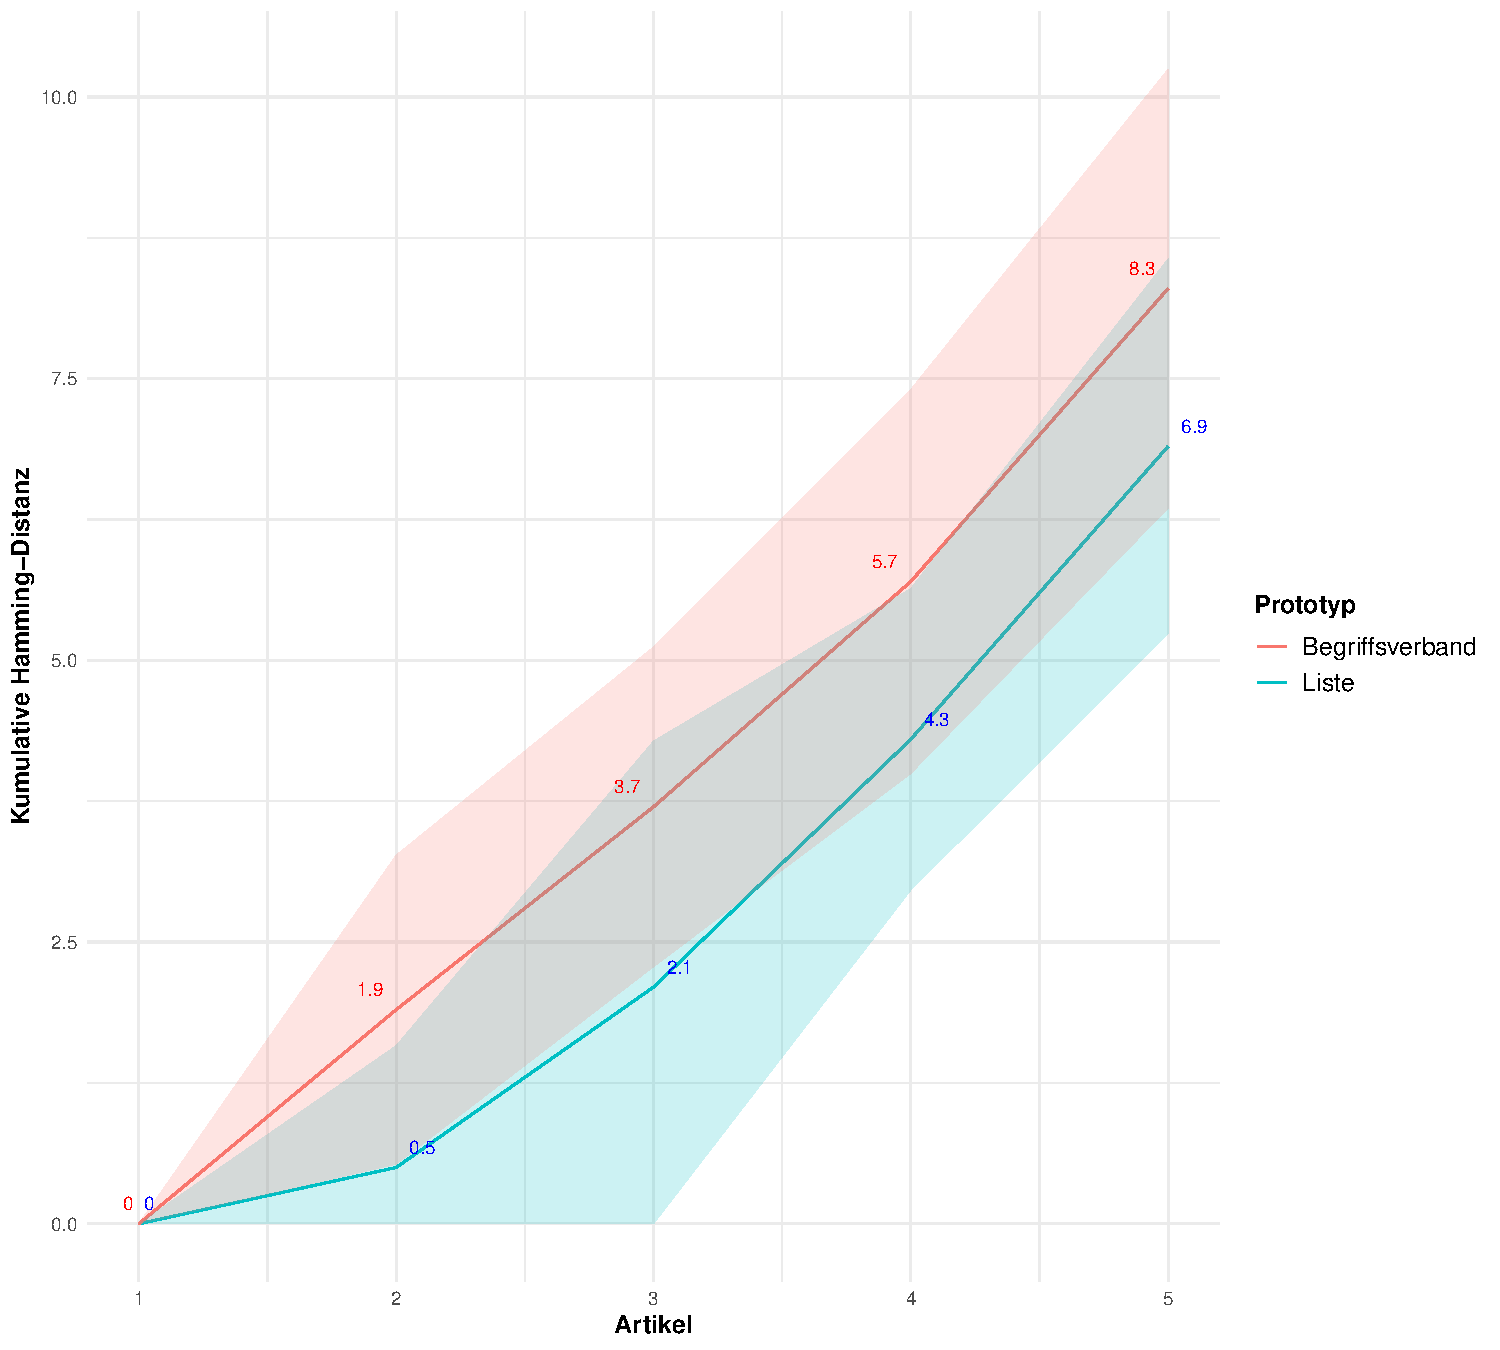
\includegraphics[width=0.8\columnwidth]{figures/comparison-line.pdf}
    \caption{\label{fig:mean-hamming}Durchschnittliche kumulative Hamming-Distanz}
\end{figure}

% Durchschnittliche Hamming-Distanz
Diese Beobachtung lässt sich deutlich bei der durchschnittlichen kumulativen Hamming-Distanz in \autoref{fig:mean-hamming} erkennen.
Die durchschnittliche kumulative Hamming-Distanz ist der Mittelwert der kumulativen Hamming-Distanz aller Testpersonen.
Der Mittelwert ist im Graphen für jeden Artikel als Text angegeben.
Das Band um die Linie stellt die Standardabweichung dar.
Dabei wurde die eine Standardabweichung, welche unter dem Wert null liegen würde nicht dargestellt.
Stattdessen werden alle Werte unter null auf null gesetzt.
Der Grund dafür ist, dass eine negative Hamming-Distanz keine sinnvolle Interpretation besitzt.
Eine negative Hamming-Distanz würde bedeuten, dass die beiden Artikel tatsächlich näher beieinander liegen als ein und derselbe Artikel.
Dies wäre ein Widerspruch, da die Hamming-Distanz die Anzahl der Positionen misst, an denen sich die beiden Artikel unterscheiden.
Daher ist der niedrigste sinnvolle Wert für die Hamming-Distanz eine Null, da diese bedeutet, dass zwei aufeinanderfolgende Artikel in Bezug auf ihre Merkmale identisch sind.\\

% Beobachtung Durchschnittliche Hamming-Distanz
In \autoref{fig:mean-hamming} ist zu erkennen, dass die durchschnittliche kumulative Hamming-Distanz für den Begriffsverband im Vergleich zur Liste in jedem Schritt höher ist.
Besonders der erste angeklickte Artikel weist eine deutlich höhere durchschnittliche kumulative Hamming-Distanz auf.
Es lässt sich ebenfalls deutlich erkennen, dass die Standardabweichung für den Begriffsverband im Regelfall über dem Mittelwert der Liste liegt.
Dies bedeutet, dass die Testpersonen bei der Navigation durch den Begriffsverband selbst nach Abweichung vom Mittelwert eine höhere Diversität aufweisen als bei der Liste.
Da zu wenige Testpersonen am Experiment teilgenommen haben, lässt sich diese Beobachtung nicht als statistisch signifikant bewerten.
Dennoch ist diese Beobachtung ein Indiz dafür, dass der Begriffsverband zu einer höheren Diversität bei der Navigation durch die Artikel führt als eine traditionelle Listendarstellung.
